\documentclass[conference]{IEEEtran}
%\IEEEoverridecommandlockouts
% The preceding line is only needed to identify funding in the first footnote. If that is unneeded, please comment it out.
\usepackage{cite}
\usepackage{amsmath,amssymb,amsfonts}
\usepackage{algorithmic}
\usepackage{graphicx}
\usepackage{textcomp}
\usepackage{xcolor}
\usepackage{cuted}
\usepackage{tikz}
\usepackage{pgfplots}


\usetikzlibrary{calc,trees,positioning,arrows,chains,shapes.geometric,%
    decorations.pathreplacing,decorations.pathmorphing,shapes,%
    matrix,shapes.symbols}

\tikzstyle{line} = [draw, -, thick]
\tikzstyle{nodraw} = [draw, fill, circle, minimum width=0pt, inner sep=0pt]
\tikzstyle{box} = [line, rectangle, rounded corners, text centered]

\tikzset{
>=stealth',
  punktchain/.style={
    rectangle, 
    rounded corners, 
    draw=black, very thick,
    text width=2em, 
    minimum height=3em, 
    text centered, 
    on chain},
  line/.style={draw, thick, <-},
  element/.style={
    tape,
    top color=white,
    bottom color=blue!50!black!60!,
    minimum width=1em,
    draw=blue!40!black!90, very thick,
    text width=2em, 
    minimum height=3.5em, 
    text centered, 
    on chain},
  every join/.style={->, thick,shorten >=1pt},
  decoration={brace},
  tuborg/.style={decorate},
  tubnode/.style={midway, right=2pt},
}


\def\BibTeX{{\rm B\kern-.05em{\sc i\kern-.025em b}\kern-.08em
    T\kern-.1667em\lower.7ex\hbox{E}\kern-.125emX}}
\newcommand*\Laplace{\mathop{}\!\mathbin\bigtriangleup}
\begin{document}

\title{Combining checkpointing and data compression\\ for high frequency seismic imaging
}

\author{\IEEEauthorblockN{Navjot Kukreja}
\IEEEauthorblockA{\textit{Department of Earth Science and Engineering} \\
\textit{Imperial College London}\\
London, UK \\
n.kukreja@imperial.ac.uk}
\and
\IEEEauthorblockN{Jan H\"uckelheim}
\IEEEauthorblockA{\textit{Department of Earth Science and Engineering}\\
\textit{Imperial College London}\\
London, UK }
\and
\IEEEauthorblockN{Mathias Louboutin}
\IEEEauthorblockA{\textit{TODO Mathias} \\
\textit{Georgia Institute of Technology}\\
Atlanta, GA, USA\\}
\and
\IEEEauthorblockN{Kaiyuan Hou}
\IEEEauthorblockA{\textit{Department of EECS} \\
\textit{Northwestern University}\\
Evanston, IL, USA \\
}
\and
\IEEEauthorblockN{5\textsuperscript{th} Given Name Surname}
\IEEEauthorblockA{\textit{dept. name of organization (of Aff.)} \\
\textit{name of organization (of Aff.)}\\
City, Country \\
email address}
\and
\IEEEauthorblockN{Gerard Gorman}
\IEEEauthorblockA{\textit{Department of Earth Science and Engineering}\\
\textit{Imperial College London}\\
London, UK }
}

\maketitle

\begin{abstract}
Full-waveform inversion is an adjoint-based optimization problem in seismic
imaging that processes terabytes of data, regularly exceeding the memory
capacity of available computers. Data compression is an effective strategy to
reduce this memory requirement by a certain factor, particularly if some loss in
accuracy is acceptable. A popular alternative is checkpointing, where data is
stored at selected points in time, and values at other times are recomputed as
needed from the last stored state.  This allows arbitrarily large adjoint
computations with limited memory, at the cost of additional recomputations.

In this paper we combine compression and checkpointing for the first
time to compute a realistic full-waveform inversion. The combination of
checkpointing and compression allows
larger adjoint computations compared to using only compression, and
reduces the recomputation overhead significantly compared to using only checkpointing.
\end{abstract}

\begin{IEEEkeywords}
component, formatting, style, styling, insert
\end{IEEEkeywords}

\section{Introduction}
The class of adjoint-based optimization problems has a very typical data access pattern where a
simulation is run ``forward" in simulation time, which produces data that is to be used by a
subsequent adjoint pass which is run backward in simulation time TODO CITE. Figure \ref{fig:dataflow}
shows the typical data access pattern. This class consists of many different problems of interest in
science and engineering. One problem in this class is full-waveform inversion (FWI) where physical
experiments are carried out by propagating seismic waves through the earth's subsurface and the
solution to the optimization problem gives the most likely structure of the earth's subsurface. Figure
\ref{fig:offshore_survey} shows the physical setup of the experiment that produces the data that this problem operates
on. The data access pattern from Figure \ref{fig:dataflow} applies here as well, since every step during the
adjoint propagation requires data from the corresponding step from the forward propagation. In
particular for FWI, this data can reach tens of terabytes in size, which is beyond the memory
available on most hardware. While this paper is written to be focussed on FWI as the target problem, 
the analysis can be applied to any problem with a similar data-access pattern. 

\begin{figure}
\begin{center}
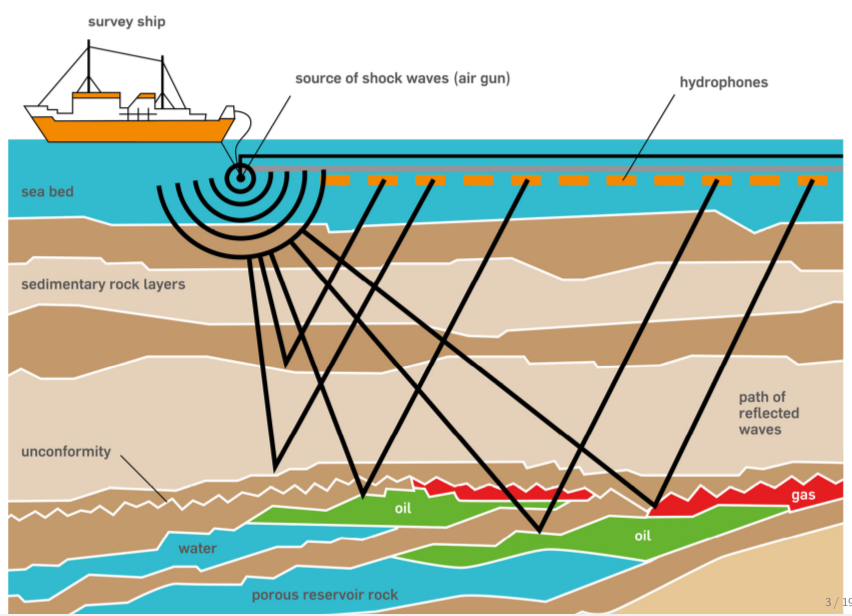
\includegraphics[width=0.8\linewidth]{images/survey-ship-diagram.png}
\end{center}
\caption{Illustration of an offshore seismic survey that collects the input data for FWI}
\label{fig:offshore_survey}
\end{figure}

Various strategies are routinely employed to reduce this memory requirement, for example 
Domain decomposition (TODO cite) where the domain of the simulation is distributed over
multiple nodes so as to fit within the memory available on each node. This introduces the overhead
of network communication and might not efficiently use the computational resources on each node.
Another common strategy, which is specific to the domain of FWI, is where only the boundaries of
the domain are stored at each timestep and the rest of the wavefield is reconstructed from the
boundaries when required (TODO CITE). Another commonly used strategy that is applied across
a much wider domain of problems is checkpointing. In this strategy, a subset of the data from the
forward pass is stored (and the rest discarded). The discarded data is recomputed when required
by rerunning the forward pass. Starting from Revolve (TODO cite), which was a provably optimal
scheduling algorithm to implement this strategy, various studies have used and extended this
technique to various scenarios (TODO cite other checkpointing papers). 

\begin{figure*}
\begin{center}
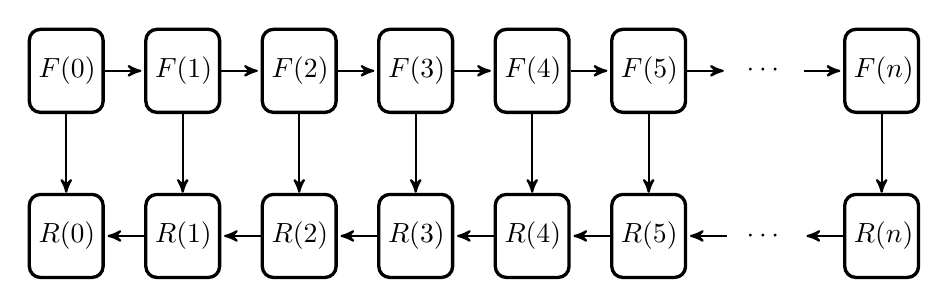
\begin{tikzpicture}
  [node distance=.5cm,
  start chain=1 going right,start chain=2 going left]
     \node[punktchain, join, on chain=1] (t1) {$F(0)$};
     \node[punktchain, join, on chain=1] (t2)      {$F(1)$};
     \node[punktchain, join, on chain=1] (t3)      {$F(2)$};
     \node[punktchain, join, on chain=1] (t4) {$F(3)$};
     \node[punktchain, join, on chain=1] (t5) {$F(4)$};
     \node[punktchain, join, on chain=1] (t6) {$F(5)$};
     \node[punktchain, join, draw=none, on chain=1] (ellipsis1) {$\cdots$};
     \node[punktchain, join, on chain=1] (tn) {$F(n)$};

\node[punktchain, below=1cm of tn, on chain=2] (atn) {$R(n)$};
\node[punktchain, join, draw=none, on chain=2] (ellipsis2) {$\cdots$};
     \node[punktchain, join, on chain=2] (at6)      {$R(5)$};
     \node[punktchain, join, on chain=2] (at5)      {$R(4)$};
     \node[punktchain, join, on chain=2] (at4) {$R(3)$};
     \node[punktchain, join, on chain=2] (at3) {$R(2)$};
     \node[punktchain, join, on chain=2] (at2) {$R(1)$};
     \node[punktchain, join, on chain=2] (at1) {$R(0)$};

\draw[|-,-|,->, thick,] (t1.south) |-+(0,-1em)-| (at1.north);
\draw[|-,-|,->, thick,] (t2.south) |-+(0,-1em)-| (at2.north);
\draw[|-,-|,->, thick,] (t3.south) |-+(0,-1em)-| (at3.north);
\draw[|-,-|,->, thick,] (t4.south) |-+(0,-1em)-| (at4.north);
\draw[|-,-|,->, thick,] (t5.south) |-+(0,-1em)-| (at5.north);
\draw[|-,-|,->, thick,] (t6.south) |-+(0,-1em)-| (at6.north);
\draw[|-,-|,->, thick,] (tn.south) |-+(0,-1em)-| (atn.north);
  \end{tikzpicture}
\end{center}
\caption{The dataflow pattern that is typical of adjoint-based optimization problems}
\label{fig:dataflow}
\end{figure*}

introduction on compression techniques - TODO Jan
Compression is an obvious addition to the tools applied to the specific data access pattern 


One possible way of using compression to speed up full-waveform inversion or any adjoint-based
optimization is by simply compressing the field data before storing it and decompressing it when it
is required again. If the memory available is sufficient to store the complete forward data after
compression, the use of compression effectively replaces the use of revolve-based checkpointing.
This scenario has been discussed in different studies before - some of which we cover in the next
section. This paper focusses on a broader region, of which this scenario is just one part. In particular,
we discuss the scenarios where the forward field can not fit in memory even after compression, where
compression and Revolve would be used in conjunction. 

Although most of the compression we discuss here introduces some error which may or may not affect
the final result of the computation, we try to avoid discussing the error in this paper and focus on the 
performance impact of compression instead.

\section{Related Work}
\cite{cyr2015towards}

\cite{dalmau2014lossy}

\cite{fichtner2009full}

\cite{gpu-compression}

\cite{boehm2016wavefield}
\cite{gpu-compression}
\cite{Kaklamanis:2012aa}

TODO cite SZ (Frank Cappello)
\section{Test case using Devito and pyRevolve}
We use Devito \cite{devito-compiler} \cite{devito-api} to setup wave equation solvers for forward and
adjoint modes. Devito is a domain-specific language to enable the rapid development of finite-difference
solvers from a high-level description of the partial differential equation. The simplest version of the wave
equation is the acoustic:
\begin{equation}
m(x)\frac{\partial^2 u(t, x)}{\partial t^2} - \Laplace u(t, x) = q(t, x)
\end{equation}
where $m(x) = \frac{1}{c^2(x)}$ is the squared slowness with $c(x)$ the spatially dependent speed of sound, 
$u(t, x)$ is the wavefield, $\Laplace u(t, x)$ denotes the laplacian of the wavefield and $q(t, x)$ is the source.
Some of the kernels used in the performance measurements corresponded to a more physically representative
but complex version of this equation called Tilted Transverse Isotropy (TTI) \cite{zhang2011stable}. We leave the 
equation itself out of this paper for brevity. 

The values of $m(x)$ were derived from the SEAM Overthrust (TODO Cite SEAM) model which was over a grid
of $287 \times 881 \times 881$ points, including an absorbing layer of 40 points on each side. The grid spacing
was TODO in space and TODO in time. This was run for TODO timesteps, and the final field stored as
representative of a typical snapshot. Figure \ref{fig:uncompressed} shows this stored field that was used for the compression tests. 

\begin{figure}
\begin{center}
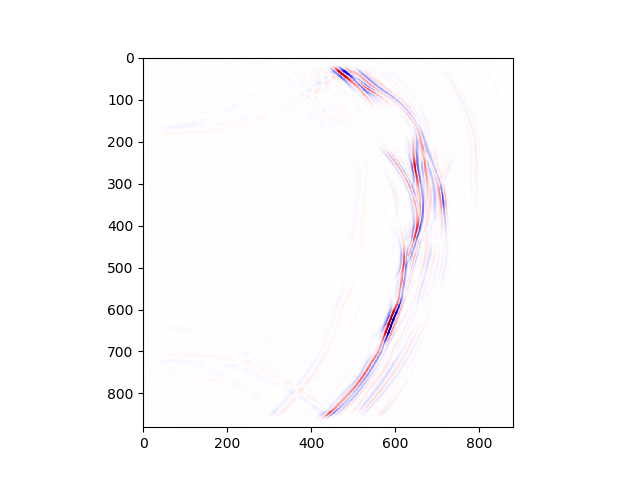
\includegraphics[width=0.8\linewidth]{images/uncompressed.png}
\end{center}
\caption{Cross-section of the wavefield used as a reference sample for compression and decompression}
\label{fig:uncompressed}
\end{figure}

To implement Revolve with Devito, we used pyRevolve (TODO CITE 2 papers) which is a python wrapper over the
original Revolve utility (TODO CITE Revolve). The performance model that will be developed in section TODO of
this paper assumes that the implementation is similar to pyRevolve, which stores a checkpoint by copying a portion
of the operator's working memory to the checkpointing memory and similarly loads a checkpoint by copying from the
checkpointing memory to the operator's working memory. Although a perfect implementation of checkpointing may
be able to avoid these copies, the overhead attached to these copies can be ignored for an operator that is
sufficiently computationally intensive. However, we include the overheads in the model to verify this assumption. 

The experiments were run on two different systems, TODO description of Richter, henceforth called Richter and a
TODO description of skylake, henceforth called Skylake.


\section{Compression algorithms}
\subsection{Lossless}
For our initial experiments, we used the python package \emph{blosc} (TODO CITE). It includes implementations for
6 different lossless compression algorithms, namely ZLIB, ZSTD, BLOSC, LZ4, LZ4HC and TODO (TODO cite all of them).
We did a parameter sweep over all available parameters to find the best-performing combinations. 
\subsection{Lossy}
Next we tried lossy compression using ZFP \cite{ratanaworabhan2006fast} (TODO verify citation). To use ZFP from python, 
we first wrote a python wrapper over the reference implementation of ZFP, which is in C. We plan to release this wrapper
in the open source community shortly. 

\begin{figure}
\begin{center}
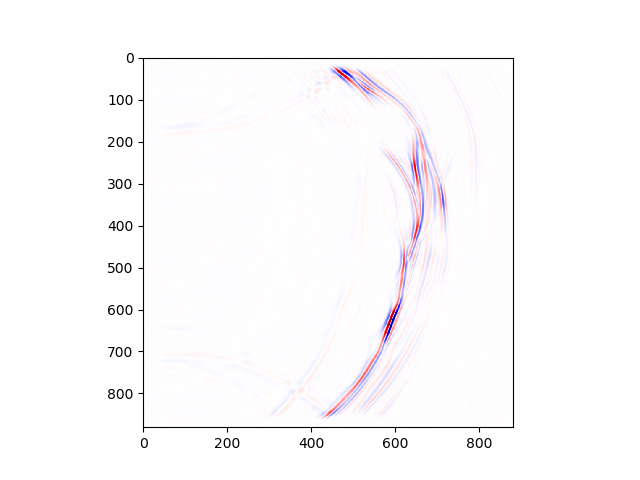
\includegraphics[width=0.8\linewidth]{images/decompressed-t-8.png}
\end{center}
\caption{Cross-section of the wavefield recovered after compression and decompression using the fixed-tolerance mode}
\label{fig:decompressed}
\end{figure}

We tried all three modes of ZFP, namely fixed-tolerance, fixed-precision and fixed-rate modes. Figure TODO shows the compression ratios
we saw for a variety of compression settings for the three modes. As expected, the highest compression efficiency was
observed in the fixed-tolerance mode albeit with highly unpredictable compression ratios. Figure \ref{fig:decompressed} shows a sample
wavefield that was recovered after compression and decompression using fixed-tolerance mode. Since, in our experiments, the time
taken to compress a checkpoint was in the same order of magnitude as the time taken to compute a timestep, we build a
performance model in the next section to evaluate the utility of compression in different scenarios of problem setups and test
platforms.



\section{Performance model for a combination of Revolve and compression}
We work with the assumption that the computation of a single forward time step takes the same wall time
as the computation of a single reverse time step - calling this $\mathbf{C}$. If the size of a single 
timestep in memory is $\mathbf{S}$ and the simulation involves $\mathbf{N}$ timesteps, the minimum
wall time required to run a single forward-adjoint evaluation is given by:
\begin{equation}
T_N = 2 \times \mathbf{C} \times \mathbf{N}
\end{equation}
However, this would require $\mathbf{S} \times \mathbf{N}$ memory. On a hardware platform where enough memory
is available, this would be the optimal strategy to compute the adjoint solution. 

When the memory available on a system is less than $\mathbf{S} \times \mathbf{N}$, Revolve provides
an optimal strategy to solve for the adjoint field by storing a subset of the $\mathbf{N}$ total checkpoints
and recomputing the remaining ones. The overhead introduced by this method can be broken down into
the recomputation overhead $\mathbf{O}_R$ and the storage overhead $\mathbf{O}_S$. The recomputation
overhead is simply the amount of time spent in recomputation, given by:
\begin{equation}
\mathbf{O}_R(N, M) = p(N, M) \cdot \mathbf{C}
\end{equation}
where $p(N, M)$ is the minimum number of recomputed steps from TODO cite revolve, reproduced
here in equation \ref{eqn:recompute}.
\begin{figure*}
\begin{equation}
\mathbf{O}_R(N, M) = \begin{cases}
      N(N-1) /2, & \text{if}\ M=1 \\
      \min\limits_{1<=\widetilde{N}<=N} \{\widetilde{N} + \mathbf{O}_R(\widetilde{N}, M) + \mathbf{O}_R(N-\widetilde{N}, M-1)\}, & \text{if}\ M>1
    \end{cases}
    \label{eqn:recompute}
\end{equation}
\end{figure*}
In equation \ref{eqn:recompute}, M is the number of checkpoints that can be stored in memory. Note that for $M >=N$, $\mathbf{O}_R$
would be zero. For $M < N$, $\mathbf{O}_R$ goes up rather quickly as M is reduced in relation to N. 

In a perfect implementation, the storage overhead $\mathbf{O}_S$ might be zero, since the computation could
be done "in-place", but in practice, checkpoints are generally stored in a separate section of memory and they
need to be transferred to a "computational" section of the memory where the compute is performed, and then
the results copied back to the checkpointing memory. This copying is a common feature of checkpointing
implementations, and might pose a non-trivial overhead in scenarios where the computation is heavily bandwidth-bound. 
This storage overhead is given by:
\begin{equation}
\mathbf{O}_SR = \mathbf{N}_W \cdot \frac{\mathbf{S}}{\mathbf{B}} + \mathbf{N}_R \times \frac{\mathbf{S}}{\mathbf{B}}
\label{eqn:storage}
\end{equation}
where $\mathbf{N}_W$ is the total number of times Revolve writes checkpoints for a single run, $ \mathbf{N}_R$ 
is the number of times checkpoints are read, and $\mathbf{B}$ is the memory bandwidth of the target system. 

The total time to solution in this scenario becomes:
\begin{equation}
T_R = 2 \times \mathbf{C} \times \mathbf{N} + \mathbf{O}_R(N, M) + \mathbf{O}_S
\end{equation}

Adding compression to the mix will increase the number of checkpoints available ($M$ in equation \ref{eqn:recompute}),
hence reducing $\mathbf{O}_R$ while adding overheads related to compression and decompression in $\mathbf{O}_S$,
as well as some error introduced by the compression. Assuming that the error remains within the allowed tolerance,
we hypothesize that, at least for some circumstances, the reduction in $\mathbf{O}_R$ should offset the increase in 
$\mathbf{O}_S$, i.e. lead to an overall decrease in the total time to solution ($T$). To build a performance model that
enables us to find the regions where compression pays off, we assume that the compression algorithm behaves uniformly
across the different time steps of the simulation, i.e. that we get the same compression ratio, compression time and 
decompression time, no matter which of the $N$ possible checkpoints we try to compress/decompress. The storage overhead
now becomes:
\begin{equation}
\mathbf{O}_SR = \mathbf{N}_W \times (\frac{\mathbf{S}}{\mathbf{F}\mathbf{B}} + t_c) + \mathbf{N}_R \times (\frac{\mathbf{S}}{\mathbf{F}\mathbf{B}} + t_d)
\end{equation}
where $\mathbf{F}$ is the compression ratio (i.e. the ratio between the uncompressed and compressed checkpoint), and $t_c$
and $t_d$ are compression and decompression times, respectively. At the same time, the recomputation overhead goes down
because $\mathbf{F}$ times more checkpoints are now available.


TODO add figure here that shows memory on x-axis and speedup on y axis. Split into 3 regions. Region 1, 
where Revolve+Compression makes sense, Region 2, where compression would probably not bring in enough benefit, 
and region 3 where compression would enable the computation to be done without revolve. 
\section{Results}


\section{Conclusions and Future work}

What are the problems?

Future work:
\begin{itemize}
\item Acceptable error bounds
\item A posteriori and a priori metrics
\item Relationship between compression error and field error, propagation of errors in forward simulation
\item Relationship between compression error and gradient error in cross-correlation
\item What else?
\end{itemize}

Disk checkpointing

\section*{Acknowledgment}

TODO (Acknowledgments for Navjot)
TODO (Acknowledgments for Jan)
TODO (Acknowledgments for Mathias)

\bibliographystyle{plain}
\bibliography{compression}

\end{document}
